\documentclass{beamer}

\usepackage[utf8]{inputenc}
\usepackage{pgfpages}
\usepackage[dvipsnames]{xcolor}
\usepackage{fancyvrb}
\usetheme{Madrid}

\definecolor{utorontoblue}{HTML}{00204e}
\colorlet{beamer@blendedblue}{utorontoblue}

\setbeamertemplate{navigation symbols}{}
% Uncomment line below for notes
%\setbeameroption{show notes on second screen}

\setbeamertemplate{note page}{\insertnote}


\title[Data Acquisition via APIs]{Data Acquisition via Application Programmable Interfaces}
\author{Adrian Petrescu}
\institute{Rubikloud}
\date{2018-10-25}

\begin{document}
\frame{\titlepage}


\begin{frame}
  \frametitle{Logistics}
  
  \begin{itemize}
    \item GitHub Repository: \href{https://github.com/apetresc/api}{https://github.com/apetresc/api}
  \end{itemize}
\end{frame}


\begin{frame}
  \frametitle{Schedule}
  
  \alert{Day 1 (Today)}
  \begin{itemize}
    \item Introduction and motivation
    \item HTTP, REST, and the languages of the web
    \item Authentication schemes
  \end{itemize}

  Day 2 (November 1st)
  \begin{itemize}
    \item Scraping unstructured data from the web
    \item Parsing 
    \item Automated spiders
  \end{itemize}

  Day 3 (November 8th)
  \begin{itemize}
    \item The server-side of APIs
    \item Deploying to the Cloud
    \item Project Description
  \end{itemize}
\end{frame}


\begin{frame}
  \frametitle{HTTP}
  \framesubtitle{Hyertext Transfer Protocol}
  \begin{itemize}
    \item The language of the web
      \note[item]{\textit{Not} the language of the internet, necessarily. There are many other protocols}
    \item Stateless
  \end{itemize}
\end{frame}


\begin{frame}
  \frametitle{Anatomy of a Request}
  \framesubtitle{Marco}
  \texttt{{\color{red}GET} {\color{darkgreen}/} {\color{blue}HTTP/1.1}}
  \pause
  \\
  \bigskip
  \\
  {
    \color{olive}
    \texttt{Host: news.ycombinator.com} \\
    \texttt{Connection: keep-alive} \\
    %\texttt{Content-Type: application/json}
    \texttt{Accept: */*}
  }
  \\
  \pause
  \bigskip
  \\
  {
    \color{violet}
    \texttt{\{ "a": "b" \}}
  }
\end{frame}


\begin{frame}
  \frametitle{Anatomy of a Response}
  \framesubtitle{Polo}

  \texttt{{\color{blue}HTTP/1.1} \color{orange}200 OK} \\
  {
    \color{olive}
    \texttt{Server: nginx} \\
    \texttt{Content-Type: text/html; charset=utf-8} \\
    \texttt{...} \\
  } \bigskip

  {
    \color{violet}
    \texttt{<html> <head> ...}
  }
\end{frame}


\begin{frame}
  \frametitle{Methods}
  \begin{itemize}
    \item \texttt{HEAD}
    \item \texttt{GET}
    \item \texttt{POST}/\texttt{PUT}
    \item \texttt{DELETE}
  \end{itemize}
\end{frame}


\begin{frame}
  \frametitle{Return Codes}
  \begin{itemize}
    \item \texttt{200} Success 
    \item \texttt{300} Redirect
    \item \texttt{400} Client Error
    \item \texttt{500} Server Error
  \end{itemize}
\end{frame}


\begin{frame}
  \frametitle{Return Codes --- \texttt{200} Success}
  \begin{itemize}
    \item \texttt{200 OK}
    \item \texttt{201 Created}
    \item \texttt{202 Accepted}
    \item \texttt{204 No Content}
    \item \texttt{206 Partial Content}
  \end{itemize}
\end{frame}


\begin{frame}
  \frametitle{Return Codes --- \texttt{300} Redirect}
  \begin{itemize}
    \item \texttt{301 Moved Permanently}
    \item \texttt{302 Moved Temporarily}
    \item \texttt{304 Not Modified}
  \end{itemize}
\end{frame}


\begin{frame}
  \frametitle{Return Codes --- \texttt{400} Client Error}
  \begin{itemize}
    \item \texttt{400 Bad Request}
    \item \texttt{401 Unauthorized}
    \item \texttt{403 Forbidden}
    \item \texttt{404 Not Found}
    \item \texttt{405 Method Not Allowed}
  \end{itemize}
\end{frame}


\begin{frame}
  \frametitle{Return Codes --- \texttt{500} Server Error}
  \begin{itemize}
    \item \texttt{500 Internal Server Error}
    \item \texttt{501 Not Implemented}
    \item \texttt{503 Service Unavailable}
  \end{itemize}
\end{frame}


\begin{frame}
  \frametitle{Authentication}
  \begin{itemize}
    \item Unauthenticated
    \item API Access Tokens
    \item OAuth 1/2
  \end{itemize}
\end{frame}


\begin{frame}[fragile=singleslide]
  \frametitle{API Access Token}
  \begin{block}{Example}
    \begin{Verbatim}[commandchars=\\\{\}]
      GET /v3/businesses/q9_gLvTNf11etVxbH7JY0Q HTTP/2
      Host: api.yelp.com
      \textcolor{red}{Authorization: Bearer p1hiON8SYR-Z[...]}
    \end{Verbatim}
  \end{block}
  
  \begin{itemize}
    \item Extremely simple to implement
    \item Only works for server-side, single-user applications
  \end{itemize}
\end{frame}


\begin{frame}
  \frametitle{OAuth}
  \begin{center}
    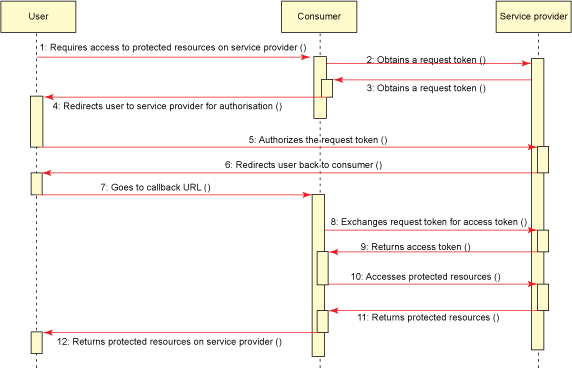
\includegraphics[width=320]{oauth-seq.png}
  \end{center}
\end{frame}


\begin{frame}
  \frametitle{Demo - Yelp}
  \begin{center}
    
\includegraphics[width=320]{yelp-logo.png}
  \end{center}
\end{frame}


\begin{frame}
  \frametitle{Demo - GitHub}
  \begin{center}
    
\includegraphics[width=320]{github-logo.png}
  \end{center}
\end{frame}

\end{document}
